  \documentclass{beamer}

% Used packages
\usepackage[utf8]{inputenc}
\usepackage[spanish]{babel}
\usepackage{amssymb, amsmath, amsthm, amsfonts, esint, mathtools}




% There are many different themes available for Beamer. A comprehensive
% list with examples is given here:
% http://deic.uab.es/~iblanes/beamer_gallery/index_by_theme.html
% You can uncomment the themes below if you would like to use a different
% one:
%\usetheme{AnnArbor}
\usetheme{Antibes}
%\usetheme{Bergen}
%\usetheme{Berkeley}
%\usetheme{Berlin}
%\usetheme{Boadilla}
%\usetheme{boxes}
%\usetheme{CambridgeUS}
%\usetheme{Copenhagen}
%\usetheme{Darmstadt}
%\usetheme{default}
%\usetheme{Frankfurt}
%\usetheme{Goettingen}
%\usetheme{Hannover}
%\usetheme{Ilmenau}
%\usetheme{JuanLesPins}
%\usetheme{Luebeck}
%\usetheme{Madrid}
%\usetheme{Malmoe}
%\usetheme{Marburg}
%\usetheme{Montpellier}
%\usetheme{PaloAlto}
%\usetheme{Pittsburgh}
%\usetheme{Rochester}
%\usetheme{Singapore}
%\usetheme{Szeged}
%\usetheme{Warsaw}

\title{Detección de Clumps en Nubes Moleculares: Un Enfoque desde el Cálculo Variacional}

% A subtitle is optional and this may be deleted
%\subtitle{Defensa de Tema de Memoria}

\author{Martín Villanueva A.\inst{1}}
% - Give the names in the same order as the appear in the paper.
% - Use the \inst{?} command only if the authors have different
%   affiliation.

\institute[Universidad Técnica Federico Santa María] % (optional, but mostly needed)
{
  \inst{1}%
  Departamento de Informática\\
  Universidad Técnica Federico Santa María}
% - Use the \inst command only if there are several affiliations.
% - Keep it simple, no one is interested in your street address.

\date{Seminario de Memoria, 2016-1}
% - Either use conference name or its abbreviation.
% - Not really informative to the audience, more for people (including
%   yourself) who are reading the slides online

%\subject{Theoretical Computer Science}
% This is only inserted into the PDF information catalog. Can be left
% out.

% If you have a file called "university-logo-filename.xxx", where xxx
% is a graphic format that can be processed by latex or pdflatex,
% resp., then you can add a logo as follows:

% \pgfdeclareimage[height=0.5cm]{university-logo}{university-logo-filename}
% \logo{\pgfuseimage{university-logo}}


% Let's get started
\begin{document}

\begin{frame}
  \titlepage
\end{frame}



\begin{frame}{Outline}
  \tableofcontents
  % You might wish to add the option [pausesections]
\end{frame}




% Section and subsections will appear in the presentation overview
% and table of contents.

\section{Objetivo General}

\begin{frame}{Objetivo General}
Realizar un análisis, estudio e implementación de un modelo basado en el \textbf{cálculo variacional}, para la
segmentación de imágenes astronómicas 3D, y de este modo poder identificar las estructuras densas (\textbf{Clumps}) que corresponden a las regiones de interés en las nubes moleculares.
\end{frame}



\section{Definición del Problema}

\subsection{Definiciones Preliminares}

\begin{frame}{Nubes Moleculares y Clumps...}
\begin{itemize}
  \item  Una \textbf{Nube Molecular} es un estructura en medio del \textit{interstellar medium}, que se caracteriza por sus bajas temperaturas y alta densidad.
  \item Están compuestas básicamente de gas y polvo ($\text{H}_2,\ \text{CO y }, \text{H}_2\text{O}$), bajo una estructura compleja compuesta de zonas de distintas densidades.
  \item La formación de estrellas se da únicamente al interior de las nubes moleculares!.
  \item Un \textbf{Clump} (\textit{cúmulo}) es entendido como una región de alta densidad contenida dentro de una nube molecular, con una fuerte emisión, acotados por alguna propiedad físico/química y de masividad variable.
  \item Entender las propiedades, estructuras y relaciones entre los clumps, ayuda a entender el proceso de formación de estrellas.  
\end{itemize}
\end{frame}

\begin{frame}{Nubes Moleculares y Clumps... (2)}
\begin{figure}[htpb!]
\centering
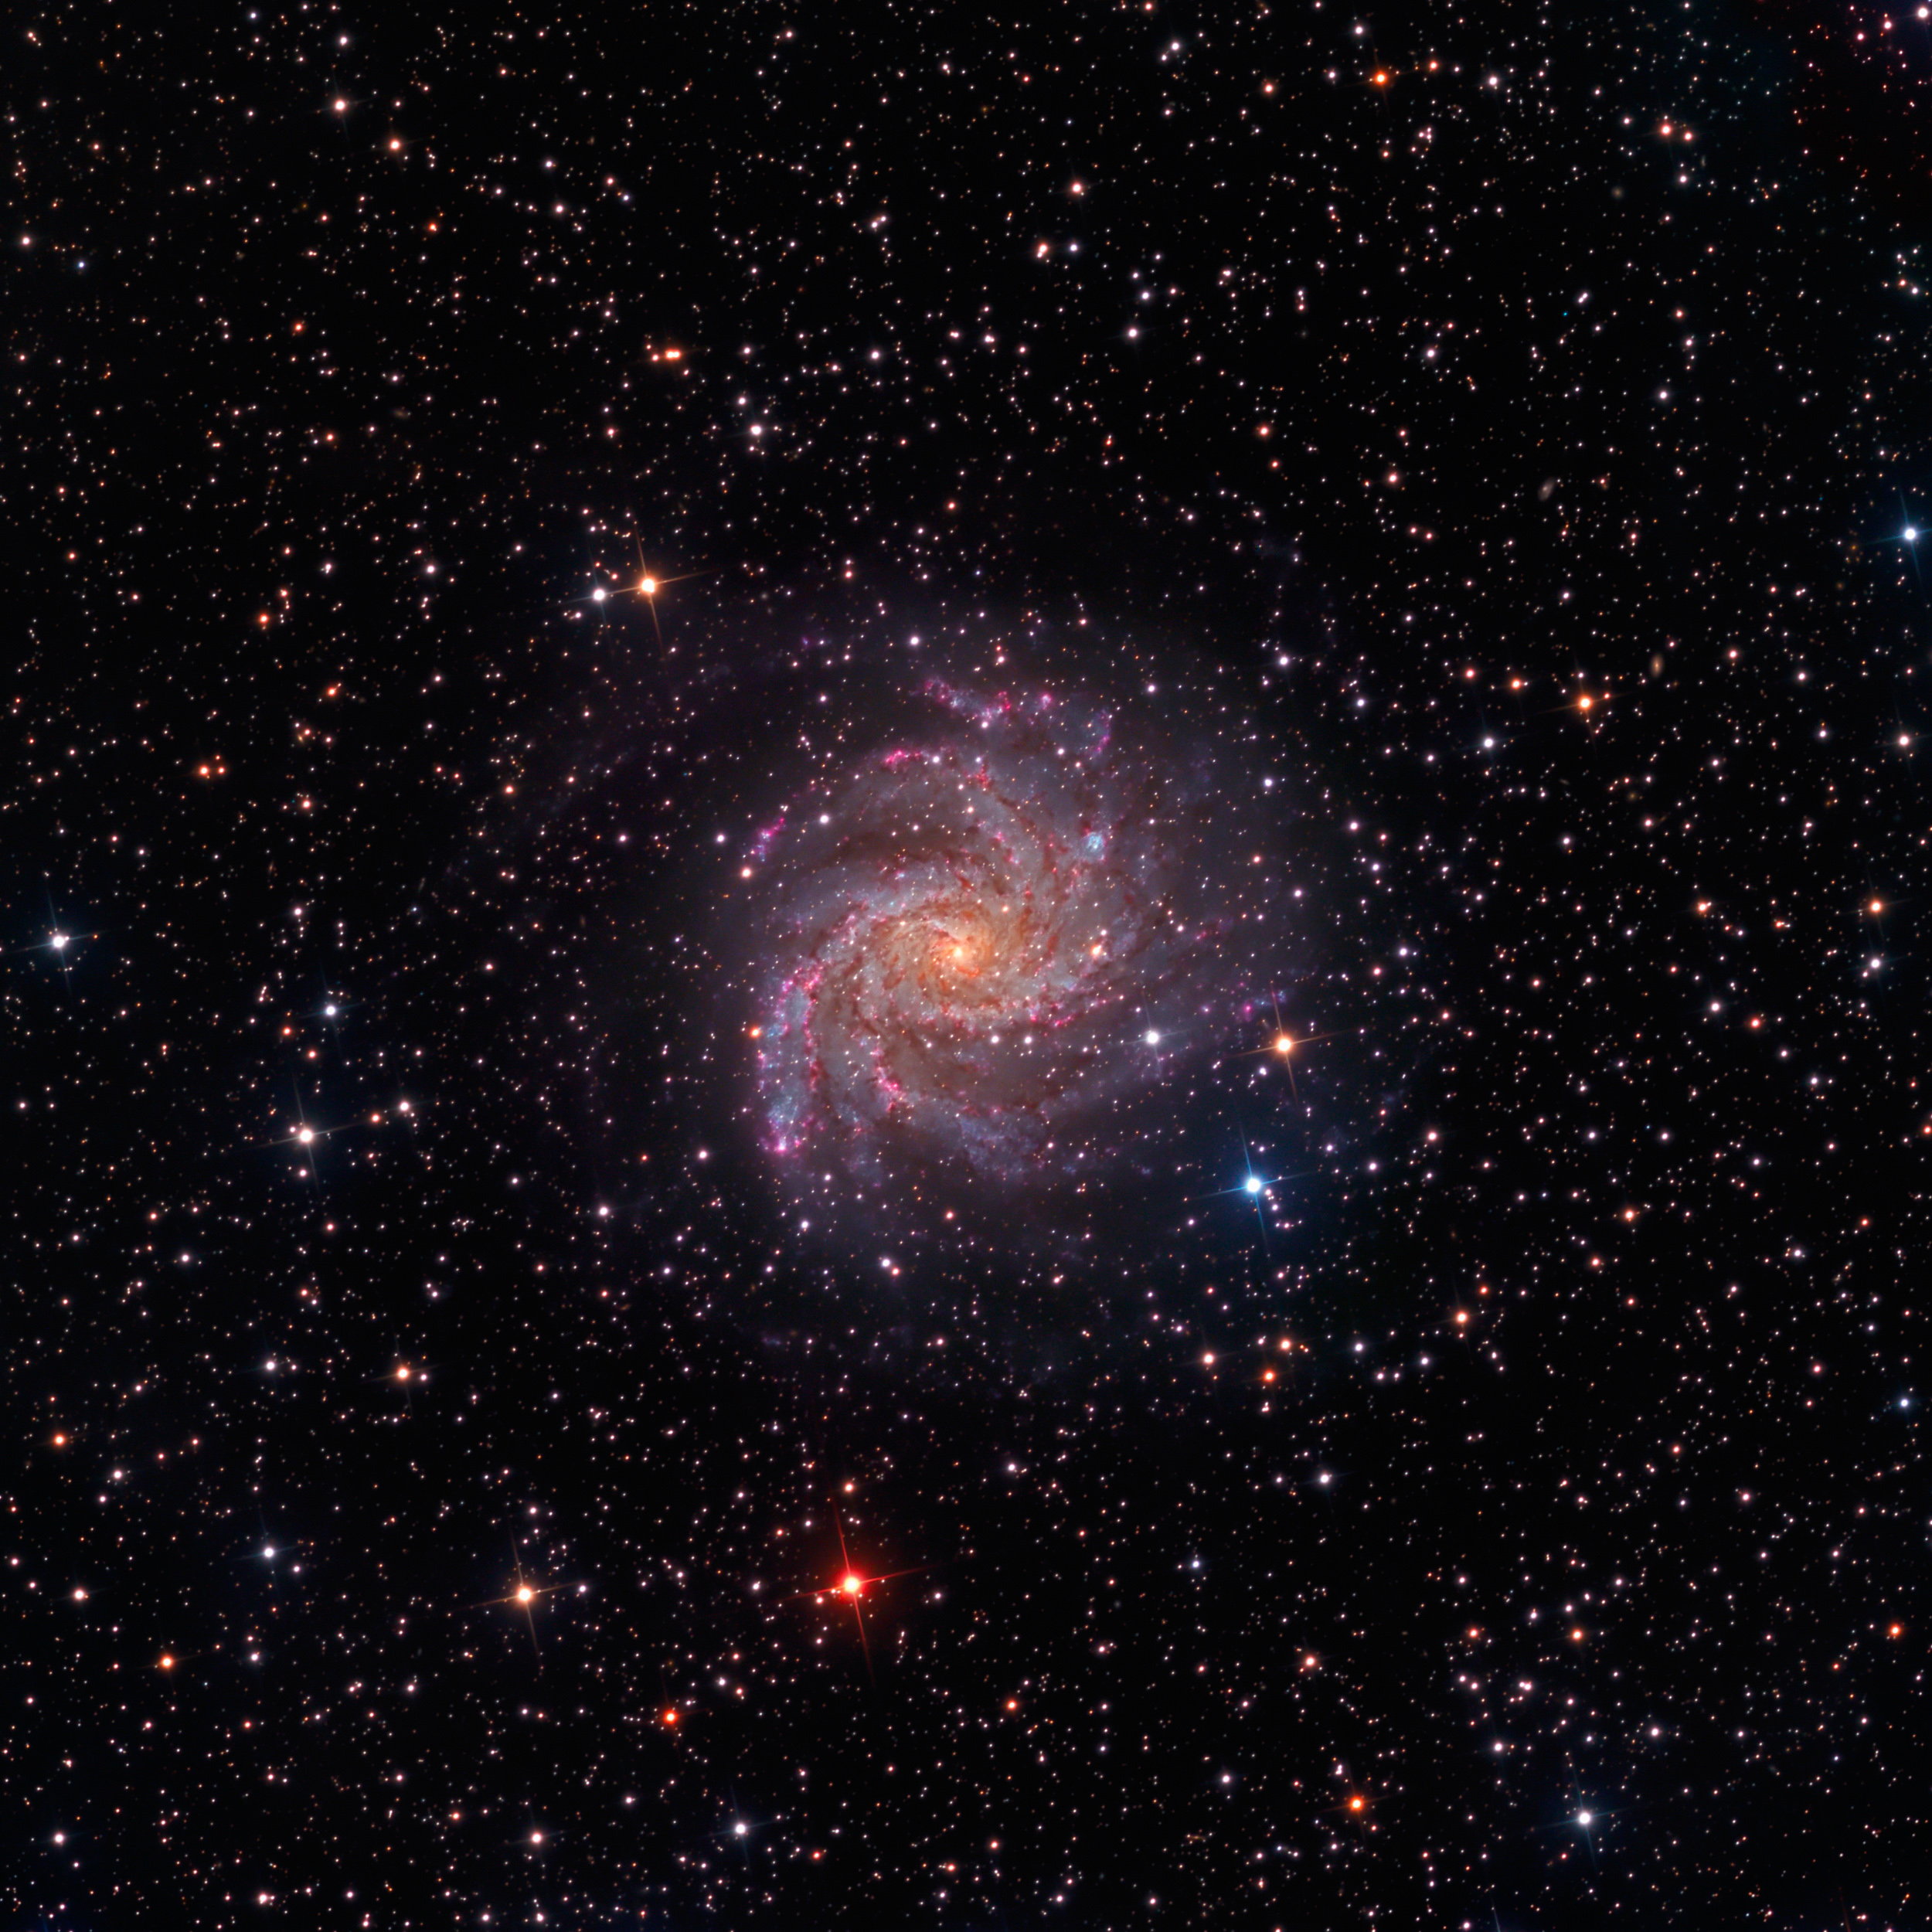
\includegraphics[width=6.7cm]{NGC6946}
\end{figure}
\end{frame}



\subsection{Cubos Espectroscópicos de Datos}
\begin{frame}{Cubos Espectroscópicos de Datos}
Los registros de las observaciones a tales nubes moleculares se almacenan en cubos de datos, que contienen
coordenadas espaciales: \textit{right ascension} y \textit{declination}, más frecuencia observada.
\begin{figure}[htpb!]
\centering
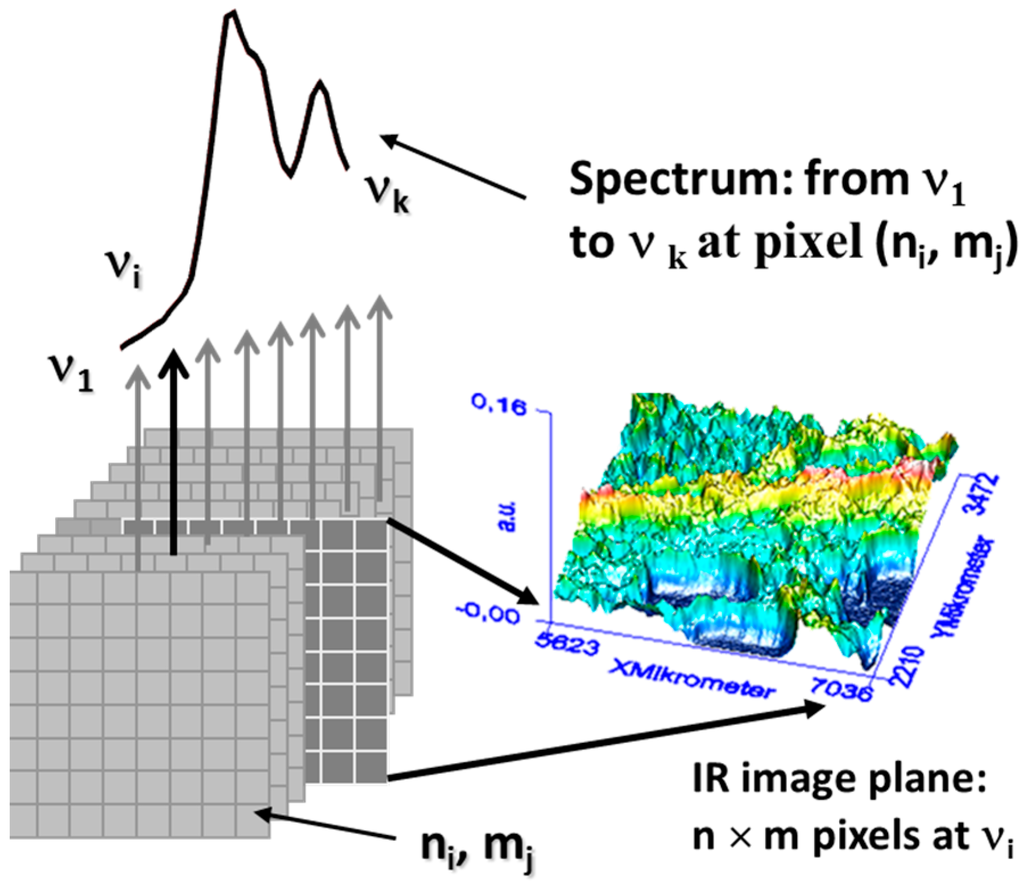
\includegraphics[width=6cm]{cube}
\end{figure}
\end{frame}



\subsection{Principales dificultades}

\begin{frame}{Principales Dificultades}
\begin{itemize}
  \item Tales imágenes astronómicas ya no pueden ser analizadas manualmente por astronomos.
  \item El tamaño de las imágenes es enorme y puede contener cientos/miles de estructuras de interés.
  \item Los cubos espectroscópicos de datos son difíciles de manipular y visualizar al día de hoy.
  \item Identificación manual sufren del \textit{bias} propio de cada astrónomo, debido a sus distintas definiciones o concepciones.
\end{itemize}

\textbf{Solución:} Construir algoritmos de detección automáticos (y deterministas), para analizar gran cantidad de datos, eliminando el juicio imparcial de cada astrónomo.  
\end{frame}





\subsection{Algoritmos de detección de Clumps}

\begin{frame}{GaussClumps [Stutzki, 1990]}
\begin{itemize}
  \item Ajustar perfiles Gaussianos a los \textit{peaks} de emisión en la data, de forma iterativa bajo un proceso de optimización.
  \item En cada iteración una Gaussiana ajustada se sustrae de la data, y se repite el proceso sobre el próximo \textit{peak} de emisión en el cubo residual.
\end{itemize}
\begin{figure}[htpb!]
\centering
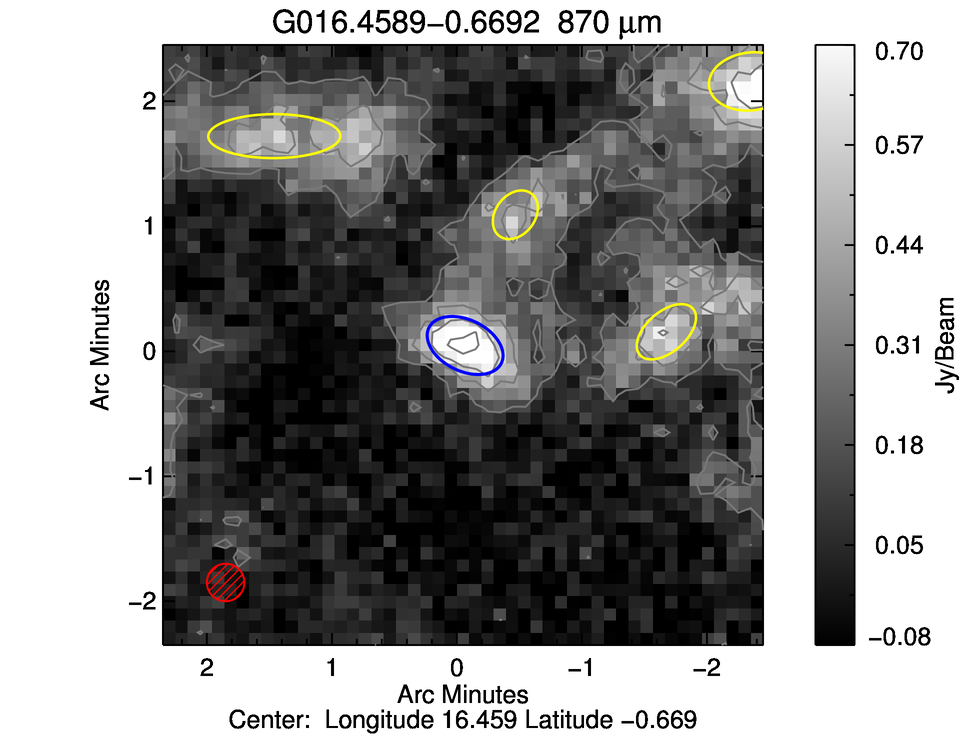
\includegraphics[width=6cm]{gc}
\end{figure}
\end{frame}


\begin{frame}{ClumpFind [Williams, 1994]}
\begin{itemize}
  \item Se analiza el cubo a distintos niveles de intensidad, partiendo desde el más alto hacia el más bajo.
  \item En cada nivel se encuentran las estructuras isoladas, y se enlazan a las estructuras vecinas del nivel superior (en caso de estar conectados).
  \item Se inspira en cómo el ojo humano segmenta las imágenes.  
\end{itemize}
\begin{figure}[htpb!]
\centering
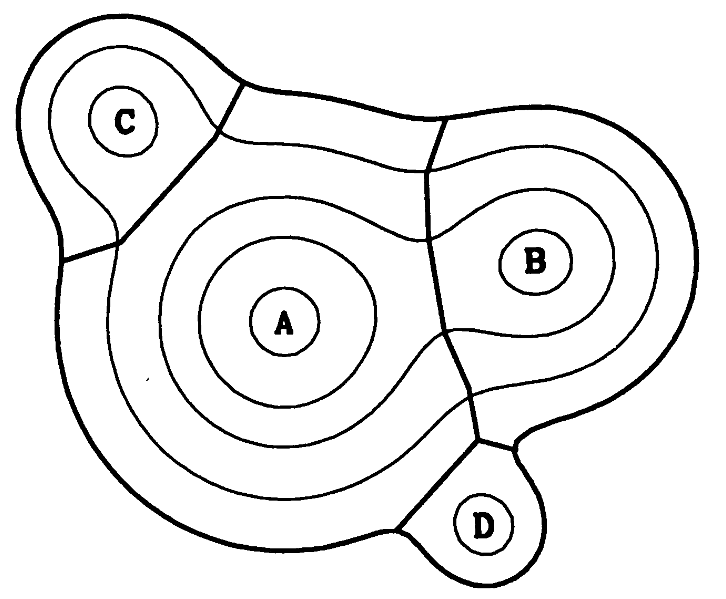
\includegraphics[width=4.5cm]{cf}
\end{figure}
\end{frame}

\begin{frame}{FellWalker [Berry, 2015]}
\begin{itemize}
  \item Algoritmo basado en \textit{Hill-Climbing}, aprovechando la propiedad de estancamiento en óptimos locales, para de esta forma definir un nuevo clump.
  \item Iterativamente computa las rutas de ascenso de mayor gradiente hasta alcanzar un \textit{peak} local, tras lo cual todos los píxeles de tal ruta son asignados a dicho \textit{clump}.
\end{itemize}
\begin{figure}[htpb!]
\centering
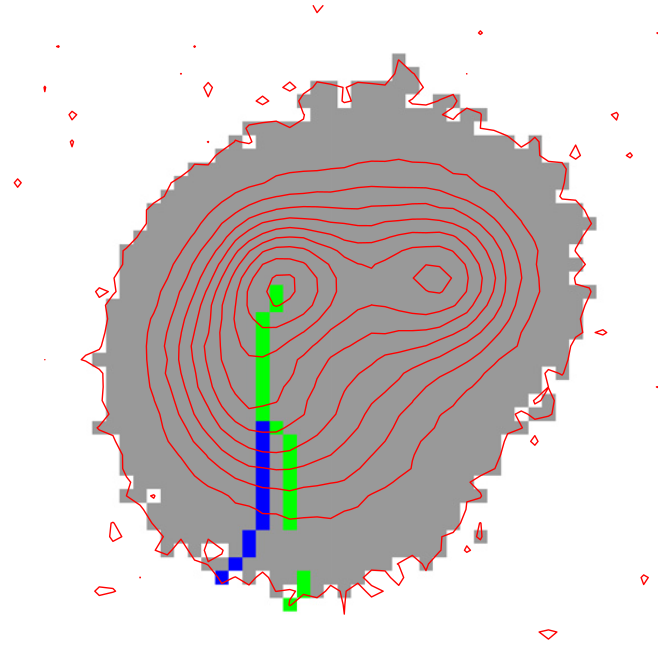
\includegraphics[width=4cm]{fw}
\end{figure}
\end{frame}

\begin{frame}{Fellwalker [Berry, 2015] (2)}
\begin{figure}[htpb!]
\centering
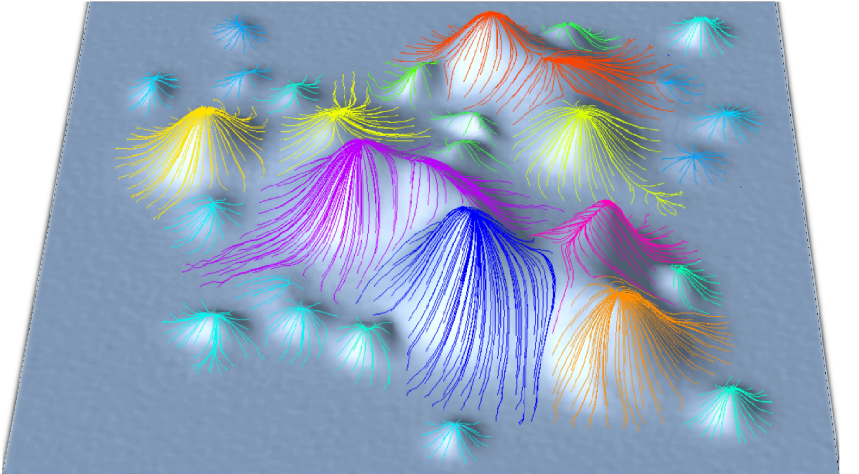
\includegraphics[width=9cm]{fw2}
\caption{Resultado Típico de FellWalker}
\end{figure}
\end{frame}

\begin{frame}{Dificultades de los Algoritmos}
En general los tres algoritmos presentados muestran los siguientes problemas:
\begin{itemize}
  \item Dependientes de una gran cantidad de parámetros, donde cada parámetro puede variar en gran medida los resultados.
  \item Varios parámetros no son simples de configurar, debido a que no tienen una interpretación física/astronómica acorde.
  \item Son computacionalmente costos y poco escalables al tamaño de la data.
\end{itemize}
\end{frame}








\section{El Enfoque Variacional}

\subsection{Definición}

\begin{frame}{Calculo Variacional}
\begin{definition}
  Sea una función $f:K^n \rightarrow K$, y el funcional $\mathcal{U}:\mathcal{F}\rightarrow K$, con $\mathcal{F}= \{f: \ f:K^n \rightarrow K \}$ un espacio de funciones. El objetivo del cálculo variacional, es determinar la función $f_0 \in \mathcal{F}$ que minimize el funcional $\mathcal{U}$:
  \begin{align*}
    \min_{f} \mathcal{U}(f) = \mathcal{U}(f_0)
  \end{align*}
  donde usualmente el funcional se expresa como una integral definida:
  \begin{align*}
    \mathcal{U}(f) = \int_{\Omega} L\left( \mathbf{x}, f(\mathbf{x}), \nabla f(\mathbf{x}), \Delta f(\mathbf{x}) \right)
  \end{align*}
  con $L$ es conocido como el \textbf{Lagrangiano}.
\end{definition}
\end{frame}

\begin{frame}{Cálculo Variacional (2)}
\begin{itemize}
  \item Siguiendo una idea similar al cálculo tradicional, es posible definir \textit{derivadas} de funcionales conocida como \textit{primera variación} o \textit{variación de Gateaux}.
  \item De este modo se traslada el problema de minimización en su forma integral, a un problema diferencial equivalente, que consiste en resolver una \textit{PDE} conocida como \textbf{Ecuación de Euler-Lagrange}.
  \item Para la resolución de esta se tienen gran cantidad de métodos numéricos (\textit{Finite Differences, Finite Element Method, Collocation Methods and Spectral Methods}).
\end{itemize}
\end{frame}

\subsection{Aplicaciones}

\begin{frame}{Cálculo Variacional en Procesamiento de Imágenes}
La filosofía del cálculo variacional en procesamiento de imágenes, es \textbf{abordar el problema de tratamiento de imágenes como si fuese un problema de aproximación de funciones}.

\begin{itemize}
  \item \textsc{Denoising}. \textbf{Objetivo}: Eliminar el ruido de una imágen. \textbf{Formulación Variacional}: Encontrar una aproximación \textit{suave} de una imagen con ruido, en el espacio de imágenes.
  \begin{figure}[htpb!]
  \centering
  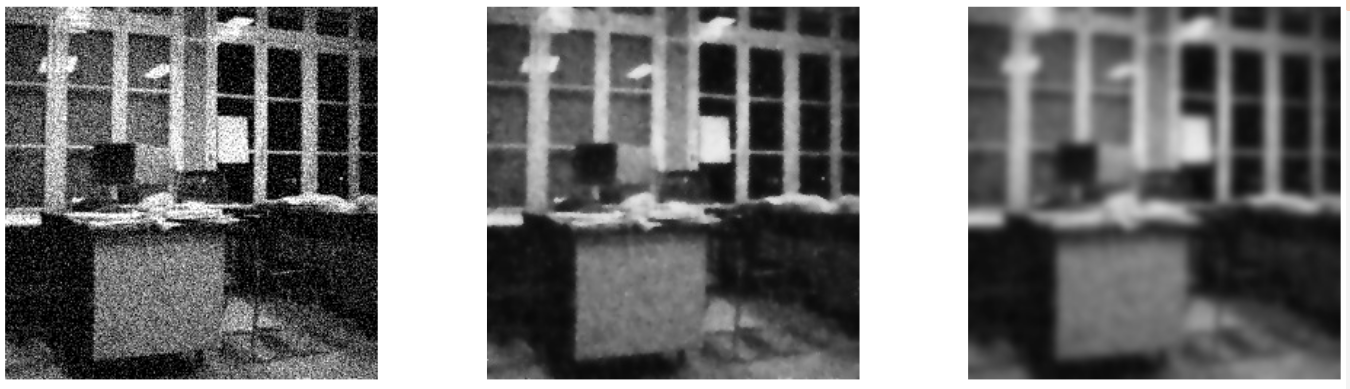
\includegraphics[width=9cm]{denoising}
  \end{figure}
\end{itemize}
\end{frame}

\begin{frame}{Cálculo Variacional en Procesamiento de Imágenes (2)}
\begin{itemize}
  \item \textsc{Restoration}. \textbf{Objetivo}: Determinar información faltante en una imagen. \textbf{Formulación Variacional}: Encontrar una aproximación de una imágen con datos faltantes, que reconstruya las zonas faltantes de modo \textit{suave}.
  \begin{figure}[htpb!]
  \centering
  
\includegraphics[width=9cm]{restoration}
  \end{figure}
\end{itemize}
\end{frame}

\begin{frame}{Cálculo Variacional en Procesamiento de Imágenes (3)}
  \begin{itemize}
      \item \textsc{Segmentation}. \textbf{Objetivo}: Particionar la imagen entre objeto y fondo. \textbf{Formulación Variacional}: Encontrar una curva cerrada \textit{suave} entre el objeto y el fondo.
    \begin{figure}[htpb!]
  \centering
  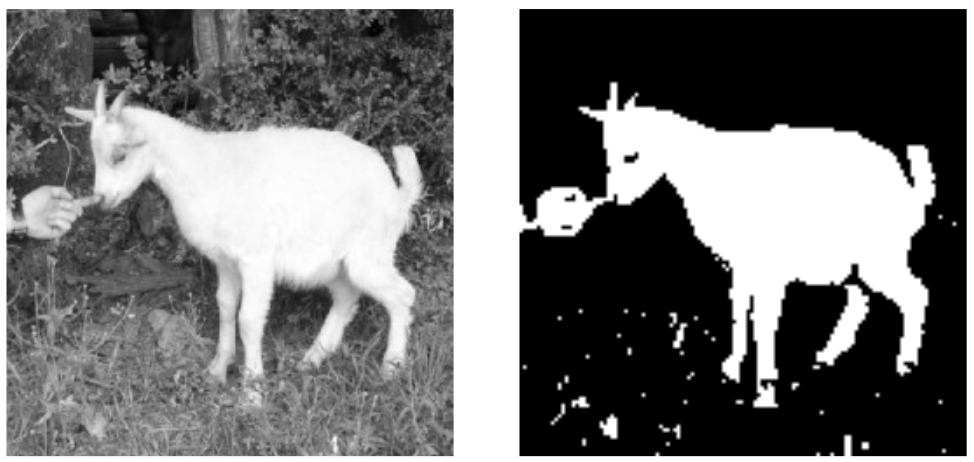
\includegraphics[width=9cm]{segmentation}
  \end{figure}
  \end{itemize}
\end{frame}


\subsection{Aplicación al problema}

\begin{frame}{Aplicación al Problema}
Sea entonces $f(x,y,z)$ la función del cubo de datos, y $u(x,y,z)$ la función que pretende aproximarla, se propone entonces el siguiente funcional:
\begin{align*} \label{eq1}
\begin{split}
\Phi(u) & = \int_{\Omega \subset R^3} L(x, y , z , u , u_x, u_y, u_z) d\Omega \\
        & = \int_{\Omega \subset R^3} F_{\text{similitud}}(f,u) + \alpha F_{\text{penalización}}(f,u)
        \\&+ \beta \ F_{\text{suavidad}}(u_x, u_y, u_z) + \cdots \ d\Omega
\end{split}
\end{align*}
Una vez planteado y definido el Lagrangiano $L$ que resuelve nuestro problema, es posible pasar a la ecuación de
\textbf{Euler-Lagrange} correspondiente.
\end{frame}


\begin{frame}{Aplicación al Problema}
Sea entonces $f(x,y,z)$ la función del cubo de datos, y $u(x,y,z)$ la función que pretende aproximarla, se propone entonces el siguiente funcional:
\begin{align*}
\begin{split}
\Phi(u) & = \int_{\Omega \subset R^3} L(x, y , z , u , u_x, u_y, u_z) d\Omega \\
        & = \int_{\Omega \subset R^3} (u-f)^2 + \alpha \Psi_1(u-f)
        \\&+ \beta \ \Psi_2( | \nabla u |^2 ) \ d\Omega
\end{split}
\end{align*}
Donde $\Psi_1$ es una función monotonamente creciente con valor $0$ para $x < 0$, y $\Psi_2$ es monotonamente creciente. 
\end{frame}


\begin{frame}{Aplicación al Problema}
Dado que no es posible trabajar en el espacio de todas las funciones $u$ posibles, y dada la estructura Gaussiana inherente de las fuentes a extraer, se propone una solución del siguiente tipo:
\begin{align*}
\begin{split}
u(\mathbf{x}) &= \sum_{i=1}^N c_i \  \text{exp}(- (\mathbf{x}-\boldsymbol{\mu}_i)^T \Sigma_i^{-1}(\mathbf{x}-\boldsymbol{\mu}_i)) \\ 
  &= \sum_{i=1}^N c_i \  \text{exp}\left(- \frac{(x - \mu_{x_i})^2 + (y - \mu_{y_i})^2 + (z - \mu_{z_i})^2}{3 \sigma_i^2} \right),
\end{split}
\end{align*}
es decir, una combinación lineal de funciones Gaussianas esféricamente simétricas, cada una parametrizada por $(\mu_{x_i}, \mu_{y_i}, \mu_{z_i}, c_i, \sigma_i)$ ($5N$ parámetros en total).
\end{frame}


\begin{frame}{Aplicación al Problema}
Para restringir el espacio de parámetros en los que opera el algoritmo de optimización, se realizan las siguientes decisiones de modelado
\begin{align*}
\begin{split}
u(\mathbf{x}) =  \sum_{i=1}^N c_i^2 \  \text{exp}\left(- \frac{(x - [\mu_{x_i} + \delta_x \sin(\theta_{x_i})])^2 + \cdots}{3 (\sigma_i + \sigma_0)^2} \right),
\end{split}
\end{align*}
donde los parámetros son ahora $(\theta_{x_i}, \theta_{y_i}, \theta_{z_i}, c_i, \sigma_i)$ ($5N$ parámetros en total). Aquí $\sigma_0$ es el \textbf{minimal broadening}, y los centros $(\mu_{x_i}, \mu_{y_i}, \mu_{z_i})$ no forma parte de los parámetros de optimización (se determinan previamente).
\end{frame}




\section{Objetivos de la Memoria}

\begin{frame}{Objetivos de la Memoria}
\begin{itemize}
  \item Determinar un modelo matemático derivado desde el cálculo variacional, que sea \textbf{consistente} con el problema a resolver, que no requiera gran \textbf{ cantidad de parámetros}, y que los parámetros a utilizar tengan una \textbf{interpretación} física/astronómica simple.
  \item Establecer un esquema para la \textbf{resolución} del problema variacional, así como las optimizaciones
  necesarias para generar un método computacionalmente eficiente, escalable y con posibilidades de
  paralelización.
  \item \textbf{Implementación} del modelo propuesto por medio del lenguaje de programación Python, haciendo uso de bibliotecas optimizadas para métodos numéricos (\textsc{NumPy, SciPy, Cython, Numba}, entre otras).
  \item Realizar un \textbf{análisis comparativo} del método aquí propuesto, con los algoritmos estándar para la detección de \textit{Clumps}.
\end{itemize}
\end{frame}

\end{document}
